\color{finishing}

\section{Konzeption}

In diesem Kapitel werden die Anforderungsdefinitionen des Projektes, mit Spezialisierung auf die verschiedenen Use Cases beschrieben.

\subsection{Anforderunsdefinitionen}

Ein Schwarmverhalten zur Interaktion von Kleinroboter benötigt verschiedene Anforderungen, um korrekt untereinander agieren zu können. Die Basis hierbei bildet das Kommunikationssystem zwischen den einzelnen Komponenten, um erfasste Daten zuverlässig zu synchronisieren. Um die Daten entsprechend zu interpretieren benötigt jede Komponente den jeweiligen Aufbau der Kommunikation, damit diese verwertet und Aktionen ausgeführt werden können.\\
Diese Aktionen repräsentieren den Grundbestandteil des Schwarmverhaltens und sind auf die verschiedenen Systeme verteilt. Die Roboter benötigen hierbei implementierte Funktionen, wie das Ansteuern von Motoren, Sensorik, sowie die Aktualisierung, um erfasste Daten an Nutzer weiterzuleiten. Zur Steuerung dient eine App für mobile Smartphones mit einem \gls{ui} um verschiedene Szenarien zu starten, sowie die Roboter kontrollieren zu können. Die Kontrollschnittstelle stellt dabei eine Desktopanwendung dar, über die der Nutzer mit den Robotern kommuniziert und Daten zur Steuerung abgreifen kann, wobei mehrere Nutzer zur selben Zeit mit verschiedenen Szenarien unterstützt werden sollen.\\

\noindent
Damit bestehen folgende Anforderungsdefinitionen an die zu erstellenden Softwarekomponenten:
\begin{itemize}
	\item Kommunikationssystem
	\item Interpretation
	\item \gls{ui}
	\item Steuerungsfunktionen
\end{itemize}

\newpage
\subsection{Softwarearchitektur}

Die Architektur des Schwarmverhaltens besteht aus drei Hauptkomponente, den Robotern, einer Desktopanwendung, sowie einer mobilen App, siehe Abbildung \ref{fig:softwarearchitecture}.\\
Diese Komponenten kommunizieren über ein drahtloses Netzwerk mittels \gls{tcp} untereinander, indem diese Zeichenketten als \gls{json} versenden. Dadurch lassen sich gesammelte Daten als Objekte kapseln und auf den verschiedenen Systemen entsprechend synchronisieren. Dies geschieht über eine Klassenstruktur, die Kommandos abbildet, durch die die kommunizierten Daten serialisiert und als Objekte dargestellt werden können.\\
Die Roboter basieren auf dem Java System \gls{lejos}, da durch die bereitgestellten Bibliotheken für \gls{ev3} Systeme eine unkomplizierte Implementierung von Logik möglich ist, sowie eine direkte Unterstützung von \gls{eclipse} gegeben ist, um erstellte Software zu debuggen. Die Roboter unterstützen für ein Schwarmverhalten klassische Funktionen, um die Daten der vorhandenen Sensorik auszulesen, sowie Motoren anzusteuern. Diese Funktionen werden einerseits durch Kommandos ausgeführt um den entsprechenden Roboter zu steuern. Anderseits werden regelmäßig Daten durch einen Prozess erfasst, um diese auf dem Backend zu aktualisieren.\\
Die App beruht auf der plattformübergreifenden Implementierung mittels des Frameworks Xamarin um möglichst viele Systeme zu erreichen. Sie baut dabei auf ein einfaches \gls{ui} mit dem Design Pattern \gls{mvvm} auf, um diese von der eigentlichen Logik zu trennen und einen qualitativ hochwertigen Quellcode zu schaffen, der einfach gewartet werden kann. Die App besitzt Basisfunktionen zur Erstellung von Kommandos, die die Verwaltung von Szenarien veranlassen und steuert somit den Schwarm.\\
Das Backend dient als Kommunikationsschnittstelle des gesamten Systems und steuert die Kommandos für den Ablauf der Szenarien. Es besitzt ein \gls{ui} mit \gls{javafx} Realisierung zur Anzeige von erfassten Daten der einzelnen Komponenten und stellt diese anhand einer auswählbaren Hierarchie dar.

\newpage
\begin{verbatim}
\end{verbatim}
\begin{figure}[h]
	\centering
	\includegraphics[width=0.65\textwidth]{images/konzeption/Softwarearchitecture.png}
	\caption{Softwarearchitektur}
	\label{fig:softwarearchitecture}
\end{figure}
\color{process}
\newpage
\subsection{Steuerung}

\begin{figure}[h]
	\centering
	\includegraphics[width=0.4\textwidth]{images/Controling.png}
	\caption{Steuerung}
	\label{fig:steuerung}
\end{figure}

\subsection{Szenarien}

Zur Steuerung der verschiedenen Roboter wurden Szenarien entwickelt. Diese repräsentieren, in welchem Kontext die teilnehmenden Roboter gesteuert werden. Dabei gibt es verschiedene Unterschiede, von Anzahl der Roboter, Nutzer, sowie des Ziels des jeweiligen Szenario. Die Steuerung der Szenarien läuft dabei jeweils gleich ab, durch die im mobilen Gerät vorhandenen Gleichgewichtssensoren, werden Parameter zur Steuerung berechnet, die für die Ausrichtung und die Geschwindigkeit des entsprechenden Roboters zuständig ist.



% Verschiedene Modi

% Bild steuerung ??

\paragraph{Control}



\paragraph{Synchron}
\paragraph{Follow}
\paragraph{Flee}
\paragraph{Catch}

\subsection{Use Cases}
\subsubsection{Connect}

\begin{figure}[h]
	\begin{center}
		\includegraphics[width=0.8\textwidth]{images/use_cases/Connect.png}
	\end{center}
	\caption{Connect}
	\label{fig:UC_Connect}
\end{figure}

\noindent
Im Use Case Connect wird eine erste Verbindung durch die Eingabe der IP-Adresse zum Backend aufgebaut. Dabei sendet die Komponente, ob Roboter oder App eine Abbildung seiner selbst als Objekt dem Backend. Daraufhin startet das Backend die Verbindung indem es der Komponente entsprechende Verbindungskommandos zusendet. Sobald eine Reaktion in einer festgelegten Zeit erfolgt, akzeptiert das Backend die Verbindung und sendet die entsprechende Id für die Komponente. Ab diesem Moment ist die Komponente verbunden und ein Robot für Aktionen entsprechend verfügbar. Die Verbindungsinitialisierung dient hierbei der Verkürzung der Reaktionszeit, die bei einem Roboter sonst entsprechend hoch wäre.

\begin{figure}[!tbp]
	\centering
	\subfloat[Connect]{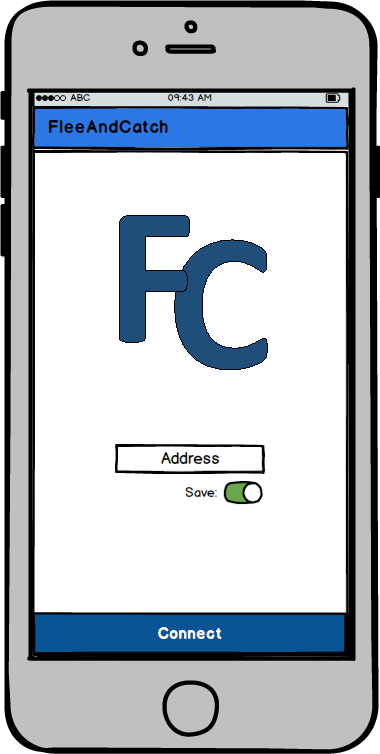
\includegraphics[width=0.4\textwidth]{images/mockups/Connection.png}\label{fig:Connect}}
	\hfill
	\subfloat[Home]{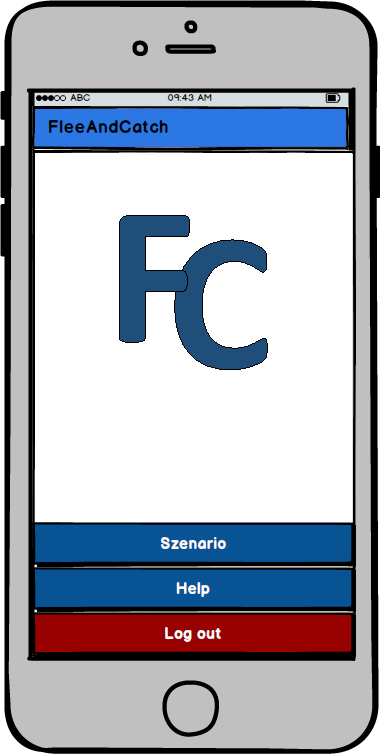
\includegraphics[width=0.4\textwidth]{images/mockups/Home.png}\label{fig:Home}}
	\caption{Connection}
\end{figure}

\subsubsection{Synchronization}

\begin{figure}[!tbp]
	\centering
	\subfloat[Update all]{\includegraphics[width=0.4\textwidth]{images/use_cases/Synchronization.png}\label{fig:UC_Synchronization}}
	\hfill
	\subfloat[Update]{\includegraphics[width=0.55\textwidth]{images/use_cases/Update.png}\label{fig:UC_Update}}
	\caption{Synchronization}
\end{figure}

\noindent
Im Use Case Synchronization werden Daten entsprechend des gesetzten Typen zwischen den Komponenten übertragen. Dabei können einerseits die Roboter als Objekte, oder ganze Szenarien übertragen werden. Dies dient zur Gegenseitigen Synchronisierung der Daten.

\begin{figure}[!tbp]
	\begin{center}
		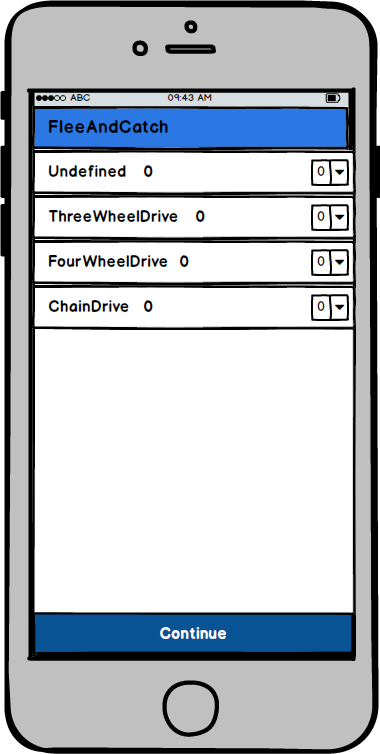
\includegraphics[width=0.5\textwidth]{images/mockups/RobotList.png}
	\end{center}
	\caption{Robot list}
	\label{fig:RobotList}
\end{figure}

\subsubsection{Szenario}

\begin{figure}[h]
	\begin{center}
		\includegraphics[width=0.6\textwidth]{images/use_cases/Spectator.png}
	\end{center}
	\caption{Spectator}
	\label{fig:UC_Spectator}
\end{figure}
\begin{figure}[h]
	\begin{center}
		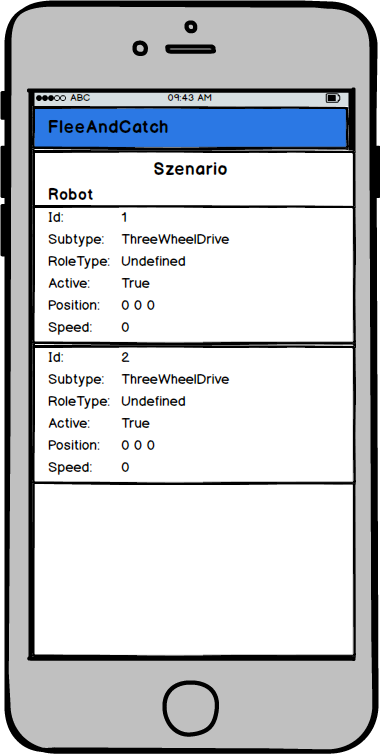
\includegraphics[width=0.6\textwidth]{images/mockups/Spectator.png}
	\end{center}
	\caption{Spectator}
	\label{fig:Spectator}
\end{figure}

\begin{figure}[h]
	\begin{center}
		\includegraphics[width=0.8\textwidth]{images/use_cases/Control.png}
	\end{center}
	\caption{Control}
	\label{fig:UC_Control}
\end{figure}
\begin{figure}[h]
	\begin{center}
		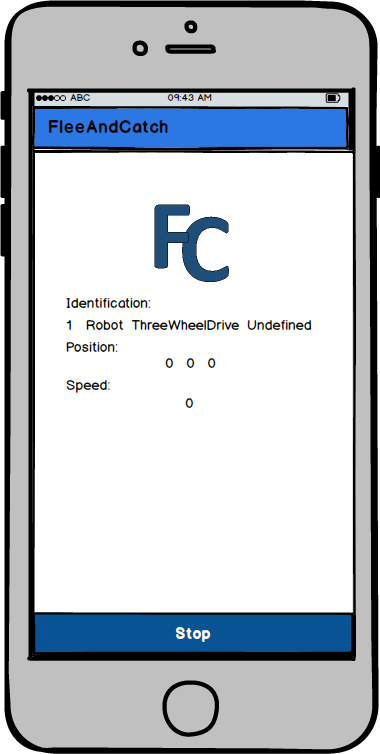
\includegraphics[width=0.6\textwidth]{images/mockups/Control.png}
	\end{center}
	\caption{Control}
	\label{fig:Control}
\end{figure}

\begin{figure}[h]
	\begin{center}
		\includegraphics[width=0.9\textwidth]{images/use_cases/Synchron.png}
	\end{center}
	\caption{Synchron}
	\label{fig:UC_Synchron}
\end{figure}

\begin{figure}[h]
	\begin{center}
		\includegraphics[width=0.9\textwidth]{images/use_cases/Follow.png}
	\end{center}
	\caption{Follow}
	\label{fig:UC_Follow}
\end{figure}

\subsubsection{Exception}
\subsection{Kommunikation}